% Options for packages loaded elsewhere
\PassOptionsToPackage{unicode}{hyperref}
\PassOptionsToPackage{hyphens}{url}
%
\documentclass[
  american,
  man,floatsintext]{apa7}
\usepackage{amsmath,amssymb}
\usepackage{lmodern}
\usepackage{ifxetex,ifluatex}
\ifnum 0\ifxetex 1\fi\ifluatex 1\fi=0 % if pdftex
  \usepackage[T1]{fontenc}
  \usepackage[utf8]{inputenc}
  \usepackage{textcomp} % provide euro and other symbols
\else % if luatex or xetex
  \usepackage{unicode-math}
  \defaultfontfeatures{Scale=MatchLowercase}
  \defaultfontfeatures[\rmfamily]{Ligatures=TeX,Scale=1}
\fi
% Use upquote if available, for straight quotes in verbatim environments
\IfFileExists{upquote.sty}{\usepackage{upquote}}{}
\IfFileExists{microtype.sty}{% use microtype if available
  \usepackage[]{microtype}
  \UseMicrotypeSet[protrusion]{basicmath} % disable protrusion for tt fonts
}{}
\makeatletter
\@ifundefined{KOMAClassName}{% if non-KOMA class
  \IfFileExists{parskip.sty}{%
    \usepackage{parskip}
  }{% else
    \setlength{\parindent}{0pt}
    \setlength{\parskip}{6pt plus 2pt minus 1pt}}
}{% if KOMA class
  \KOMAoptions{parskip=half}}
\makeatother
\usepackage{xcolor}
\IfFileExists{xurl.sty}{\usepackage{xurl}}{} % add URL line breaks if available
\IfFileExists{bookmark.sty}{\usepackage{bookmark}}{\usepackage{hyperref}}
\hypersetup{
  pdftitle={Study 1},
  pdfauthor={Blinded1, Blinded2, Blinded1, \& Blinded1},
  pdflang={en-US},
  pdfkeywords={keywords},
  hidelinks,
  pdfcreator={LaTeX via pandoc}}
\urlstyle{same} % disable monospaced font for URLs
\usepackage{graphicx}
\makeatletter
\def\maxwidth{\ifdim\Gin@nat@width>\linewidth\linewidth\else\Gin@nat@width\fi}
\def\maxheight{\ifdim\Gin@nat@height>\textheight\textheight\else\Gin@nat@height\fi}
\makeatother
% Scale images if necessary, so that they will not overflow the page
% margins by default, and it is still possible to overwrite the defaults
% using explicit options in \includegraphics[width, height, ...]{}
\setkeys{Gin}{width=\maxwidth,height=\maxheight,keepaspectratio}
% Set default figure placement to htbp
\makeatletter
\def\fps@figure{htbp}
\makeatother
\setlength{\emergencystretch}{3em} % prevent overfull lines
\providecommand{\tightlist}{%
  \setlength{\itemsep}{0pt}\setlength{\parskip}{0pt}}
\setcounter{secnumdepth}{-\maxdimen} % remove section numbering
% Make \paragraph and \subparagraph free-standing
\ifx\paragraph\undefined\else
  \let\oldparagraph\paragraph
  \renewcommand{\paragraph}[1]{\oldparagraph{#1}\mbox{}}
\fi
\ifx\subparagraph\undefined\else
  \let\oldsubparagraph\subparagraph
  \renewcommand{\subparagraph}[1]{\oldsubparagraph{#1}\mbox{}}
\fi
% Manuscript styling
\usepackage{upgreek}
\captionsetup{font=singlespacing,justification=justified}

% Table formatting
\usepackage{longtable}
\usepackage{lscape}
% \usepackage[counterclockwise]{rotating}   % Landscape page setup for large tables
\usepackage{multirow}		% Table styling
\usepackage{tabularx}		% Control Column width
\usepackage[flushleft]{threeparttable}	% Allows for three part tables with a specified notes section
\usepackage{threeparttablex}            % Lets threeparttable work with longtable

% Create new environments so endfloat can handle them
% \newenvironment{ltable}
%   {\begin{landscape}\begin{center}\begin{threeparttable}}
%   {\end{threeparttable}\end{center}\end{landscape}}
\newenvironment{lltable}{\begin{landscape}\begin{center}\begin{ThreePartTable}}{\end{ThreePartTable}\end{center}\end{landscape}}

% Enables adjusting longtable caption width to table width
% Solution found at http://golatex.de/longtable-mit-caption-so-breit-wie-die-tabelle-t15767.html
\makeatletter
\newcommand\LastLTentrywidth{1em}
\newlength\longtablewidth
\setlength{\longtablewidth}{1in}
\newcommand{\getlongtablewidth}{\begingroup \ifcsname LT@\roman{LT@tables}\endcsname \global\longtablewidth=0pt \renewcommand{\LT@entry}[2]{\global\advance\longtablewidth by ##2\relax\gdef\LastLTentrywidth{##2}}\@nameuse{LT@\roman{LT@tables}} \fi \endgroup}

% \setlength{\parindent}{0.5in}
% \setlength{\parskip}{0pt plus 0pt minus 0pt}

% Overwrite redefinition of paragraph and subparagraph by the default LaTeX template
% See https://github.com/crsh/papaja/issues/292
\makeatletter
\renewcommand{\paragraph}{\@startsection{paragraph}{4}{\parindent}%
  {0\baselineskip \@plus 0.2ex \@minus 0.2ex}%
  {-1em}%
  {\normalfont\normalsize\bfseries\itshape\typesectitle}}

\renewcommand{\subparagraph}[1]{\@startsection{subparagraph}{5}{1em}%
  {0\baselineskip \@plus 0.2ex \@minus 0.2ex}%
  {-\z@\relax}%
  {\normalfont\normalsize\itshape\hspace{\parindent}{#1}\textit{\addperi}}{\relax}}
\makeatother

% \usepackage{etoolbox}
\makeatletter
\patchcmd{\HyOrg@maketitle}
  {\section{\normalfont\normalsize\abstractname}}
  {\section*{\normalfont\normalsize\abstractname}}
  {}{\typeout{Failed to patch abstract.}}
\patchcmd{\HyOrg@maketitle}
  {\section{\protect\normalfont{\@title}}}
  {\section*{\protect\normalfont{\@title}}}
  {}{\typeout{Failed to patch title.}}
\makeatother
\keywords{keywords\newline\indent Word count: TBC}
\usepackage{csquotes}
\raggedbottom
\ifxetex
  % Load polyglossia as late as possible: uses bidi with RTL langages (e.g. Hebrew, Arabic)
  \usepackage{polyglossia}
  \setmainlanguage[variant=american]{english}
\else
  \usepackage[main=american]{babel}
% get rid of language-specific shorthands (see #6817):
\let\LanguageShortHands\languageshorthands
\def\languageshorthands#1{}
\fi
\ifluatex
  \usepackage{selnolig}  % disable illegal ligatures
\fi
\newlength{\cslhangindent}
\setlength{\cslhangindent}{1.5em}
\newlength{\csllabelwidth}
\setlength{\csllabelwidth}{3em}
\newenvironment{CSLReferences}[2] % #1 hanging-ident, #2 entry spacing
 {% don't indent paragraphs
  \setlength{\parindent}{0pt}
  % turn on hanging indent if param 1 is 1
  \ifodd #1 \everypar{\setlength{\hangindent}{\cslhangindent}}\ignorespaces\fi
  % set entry spacing
  \ifnum #2 > 0
  \setlength{\parskip}{#2\baselineskip}
  \fi
 }%
 {}
\usepackage{calc}
\newcommand{\CSLBlock}[1]{#1\hfill\break}
\newcommand{\CSLLeftMargin}[1]{\parbox[t]{\csllabelwidth}{#1}}
\newcommand{\CSLRightInline}[1]{\parbox[t]{\linewidth - \csllabelwidth}{#1}\break}
\newcommand{\CSLIndent}[1]{\hspace{\cslhangindent}#1}

\title{Study 1}
\author{Blinded\textsuperscript{1}, Blinded\textsuperscript{2}, Blinded\textsuperscript{1}, \& Blinded\textsuperscript{1}}
\date{}


\shorttitle{Cognitive Load and Moral Dumbfounding}

\authornote{

Correspondence concerning this article should be addressed to Blinded, Blinded. E-mail: Blinded

}

\affiliation{\vspace{0.5cm}\textsuperscript{1} Blinded\\\textsuperscript{2} Blinded}

\abstract{
Six studies etc.
}



\begin{document}
\maketitle

\hypertarget{study-1---college-sample}{%
\section{Study 1 - College Sample}\label{study-1---college-sample}}

The aim of Study 1 was to investigate if a cognitive load manipulation influenced participants' ability to justify their judgement. We also measured Need for Cognition (Cacioppo \& Petty, 1982; Petty et al., 1984) as a potential moderator variable.

\hypertarget{study-1-method}{%
\subsection{Study 1: Method}\label{study-1-method}}

\hypertarget{study-1-participants-and-design}{%
\subsubsection{Study 1: Participants and design}\label{study-1-participants-and-design}}

Study 1 was a between subjects design. The dependent variable was rates of providing reasons/dumbfounding (measured using to the critical slide with 3 response options: 1: providing reasons; 2: there is nothing wrong; 3: dumbfounded response - admission). The independent variable was cognitive load with two levels: present and absent. Cognitive load was manipulated by presenting participants with an eight digit number letter string to be memorized. Need for Cognition (Cacioppo \& Petty, 1982; Petty et al., 1984) was included as an additional potential predictor variable.

A total sample of 66 participants (55 female, 11 male; \emph{M}\textsubscript{age} = 22.42, min = 18, max = 57, \emph{SD} = 6.86) took part. Participants in this sample were undergraduate students, postgraduate students, and alumni from Mary Immaculate College (MIC), and University of Limerick (UL). Participation was voluntary and participants were not reimbursed for their participation.

\hypertarget{study-1-procedure-and-materials}{%
\subsubsection{Study 1: Procedure and materials}\label{study-1-procedure-and-materials}}

Data were collected using an online questionnaire. Data collection took place in a designated computer laboratory in MIC. The experimenter remained in the laboratory for the duration of the study. Participants were first presented with an information sheet and consent form. The main study proceeded when participants had signed the consent form.

Participants in the experimental condition were presented with an eight digit number/letter string and asked to memorise the sequence. After 30 seconds, the experiment progressed to the next slide. Participants had the option to click ``ok'' and progress to the next slide after 15 seconds.

Participants were then presented with the ``Julie and Mark'' (\emph{Incest}) vignette (Haidt, Björklund, \& Murphy, 2000). Participants rated on a 7-point Likert scale how right or wrong the behaviour of Julie and Mark was (where, 1 = \emph{Morally wrong}; 4 = \emph{neutral}; 7 = \emph{Morally right}), and were given an opportunity to provide reasons for their judgement. Following this, participants were presented with a series of counter-arguments, which refuted commonly used justifications for rating the behaviour as ``wrong.''

Dumbfounding was measured using the critical slide (McHugh et al., 2017). This contained a statement defending the behaviour and a question as to how the behaviour could be wrong (``Julie and Mark's behaviour did not harm anyone, how can there be anything wrong with what they did?''). There were three possible answer options: (a) ``There is nothing wrong''; (b) an admission of not having reasons (``It's wrong but I can't think of a reason''); and finally a judgement with accompanying justification (c) ``It's wrong and I can provide a valid reason.'' The order of these response options was randomised. Participants who selected (c) were prompted to type a reason. The selecting of option (b), the admission of not having reasons, was taken to be a dumbfounded response. We note that this measure provides a conservative measure of dumbfounded responding (see McHugh et al., 2017 for discussion).

Following the critical slide, participants in the experimental condition were required to reproduce the eight digit number-letter string sequence presented previously. Following this a post-discussion questionnaire in which participants rated their response to the scenario across various dimensions (Haidt, Björklund, \& Murphy, 2000).

Need for Cognition was measured using the short form of the Need for Cognition scale (Cacioppo \& Petty, 1982; Petty et al., 1984). This is an 18 item scale containing questions relating to motivation to engage in thinking (e.g., ``I would prefer complex to simple problems''). Responses were recorded on a -4 to +4 Likert-type scale, where -4 = \emph{very strong disagreement} and +4 = \emph{very strong agreement}.

\hypertarget{study-1-results}{%
\subsection{Study 1: Results}\label{study-1-results}}

Forty six participants (69.70\%) rated the behavior of Julie and Mark as wrong initially, and forty one participants (62.12\%) rated the behavior as wrong at the end of the task. Initial ratings (\emph{M} = 2.38, \emph{SD} = 1.87) were significantly more severe than revised ratings (\emph{M} = 2.82, \emph{SD} = 1.91), \emph{t}(65) = -3.03, \emph{p} = .004; \emph{d} = 0.37. Inspection of the binned judgments revealed that twelve participants changed the valence of their judgments, and all but one of these involved included a ``neutral'' response for either the initial judgment or revised judgment (see Supplementary materials Table XX).

Participants who selected the admission of not having reasons on the critical slide were identified as dumbfounded. Thirteen participants (19.70\%) selected ``It's wrong but I can't think of a reason.'' Thirty three participants (50\%) selected ``It's wrong and I can provide a valid reason''; and twenty participants (30.30\%) selected ``There is nothing wrong.''

\begin{figure}
\centering
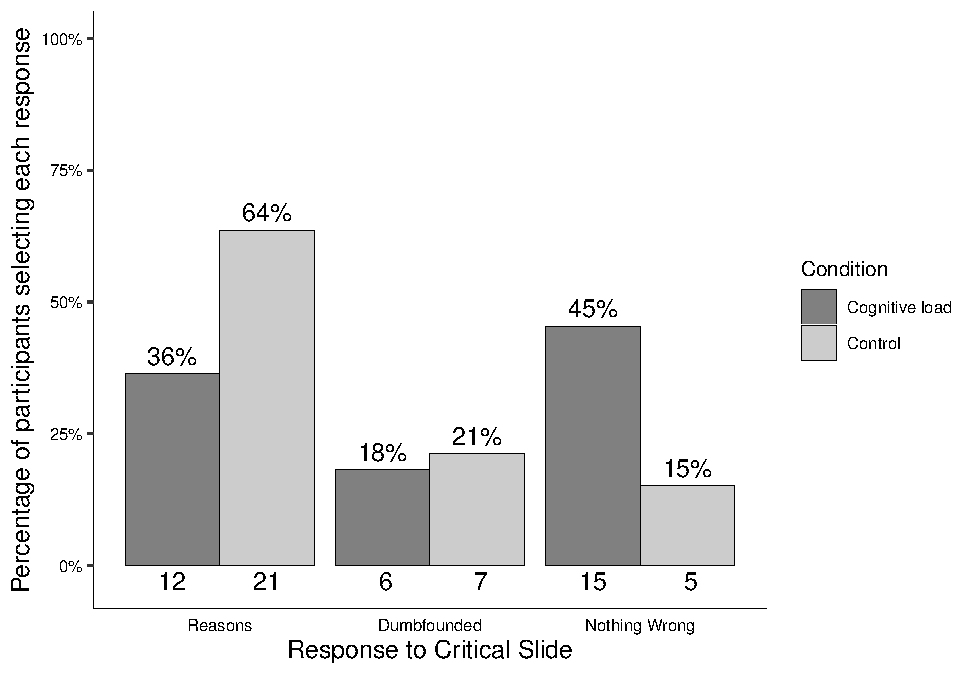
\includegraphics{Study_1_files/figure-latex/S1S1fig2criticalcondition-1.pdf}
\caption{\label{fig:S1S1fig2criticalcondition}Study 1: Responses to critical slide and for the experimental group (\emph{N} = 33) and the control group (\emph{N} = 33)}
\end{figure}

Regarding the cognitive load manipulation, nine participants (27.27\%) successfully remembered the sequence of numbers and letters in full, and five participants (15.15\%) indicated they found the memory task easy. Of these, four participants both found the task easy and got the answer right. All participants correctly remembered at least two digits, indicating at least some level of engagement with the cognitive load manipulation. There were no differences in initial judgement, \emph{t}(63.90) = 1.26, \emph{p} = .214; \emph{d} = 0.31, or revised judgment, \emph{t}(63.99) = 1.16, \emph{p} = .250; \emph{d} = 0.29, depending on cognitive load.

To test our main hypotheses we conducted a chi-squared test for independence which revealed a significant association between experimental condition and response to the critical slide, \(\chi\)\textsuperscript{2}(2, \emph{N} = 66) = 7.53, \emph{p} = .023, \emph{V} = 0.34, the observed power was 0.69. Under cognitive load fewer participants (12; 36.36\%) provided reasons than in the control condition (21; 63.64\%). Similarly, under cognitive load more participants (15; 45.45\%) selected ``There is nothing wrong'' than in the control group (5; 15.15\%). The responses to the critical slide for the experimental group (\emph{N} = 33) and the control group (\emph{N} = 33) are displayed in Figure~\ref{fig:S1S1fig2criticalcondition}. The observed counts, expected counts and standardised residuals are displayed in Table~\ref{tab:S1tab1dumb}.

\begin{table}[tbp]

\begin{center}
\begin{threeparttable}

\caption{\label{tab:S1tab1dumb}Study 1 – Observed counts, expected counts, and standardised residuals for each response to the critical slide depending on cognitive load}

\begin{tabular}{llcc}
\toprule
 & \multicolumn{1}{c}{} & \multicolumn{1}{c}{Cognitive Load} & \multicolumn{1}{c}{Control}\\
\midrule
Observed count & Reasons & 12 & 21\\
 & Dumbfounded & 6 & 7\\
 & Nothing Wrong & 15 & 5\\
Expected count & Reasons & 16.5 & 16.5\\
 & Dumbfounded & 6.5 & 6.5\\
 & Nothing Wrong & 10 & 10\\
Standardised residuals & Reasons & -2.22* & 2.22*\\
 & Dumbfounded & -0.31 & 0.31\\
 & Nothing Wrong & 2.68* & -2.68*\\
\bottomrule
\addlinespace
\end{tabular}

\begin{tablenotes}[para]
\normalsize{\textit{Note.} * = sig. at \emph{p} < .05; ** = sig. at \emph{p} < .001}
\end{tablenotes}

\end{threeparttable}
\end{center}

\end{table}

A multinomial logistic regression revealed no significant association between Need for Cognition and response to the critical slide, \(\chi\)\textsuperscript{2}(2, \emph{N} = 66) = 4.86, \emph{p} = .088, the observed power was 0.49.

\hypertarget{refs}{}
\begin{CSLReferences}{1}{0}
\leavevmode\hypertarget{ref-cacioppo_need_1982}{}%
Cacioppo, J. T., \& Petty, R. E. (1982). The need for cognition. \emph{Journal of Personality and Social Psychology}, \emph{42}(1), 116--131. \url{https://doi.org/10.1037/0022-3514.42.1.116}

\leavevmode\hypertarget{ref-haidt_moral_2000}{}%
Haidt, J., Björklund, F., \& Murphy, S. (2000). Moral dumbfounding: When intuition finds no reason. \emph{Unpublished Manuscript, University of Virginia}.

\leavevmode\hypertarget{ref-mchugh_searching_2017a}{}%
McHugh, C., McGann, M., Igou, E. R., \& Kinsella, E. L. (2017). Searching for {Moral Dumbfounding}: Identifying {Measurable Indicators} of {Moral Dumbfounding}. \emph{Collabra: Psychology}, \emph{3}(1), 1--24. \url{https://doi.org/10.1525/collabra.79}

\leavevmode\hypertarget{ref-petty_efficient_1984}{}%
Petty, R. E., Cacioppo, J. T., \& Kao, C. F. (1984). The efficient assessment of need for cognition. \emph{Journal of Personality Assessment}, \emph{48}(3), 306--307.

\end{CSLReferences}


\end{document}
